\chapter{Guidelines}\label{chapter:guidelines}
\section{Context}\label{section:guidelines/context}
The major objective of the research is to devise some guidelines so that the task of approaching any complex problem domain using microservices architectural approach becomes easier. Additionally, a few research questions related to crucial topics on microservices have emerged. The research questions are taken as stepping stones for discovering guidelines.
\\
At first, the concept related to the granularity of the microservices is studied in detail in Chapter \ref{chapter:granularity}. In this chapter, the semantic meaning of the size along with various dimensions defining granularity are discussed. Finally, various principles to evaluate the optimum size for microservices are listed.
\\
Secondly, other quality attributes to be considered when designing good microservices are listed in Chapter \ref{chapter:quality_of_service}. The quality metrics to determine each of these quality attributes are also mentioned. The various quality metrics lead to a limited list of basic metrics. Finally, various principles to determine quality of good services along with the way the quality attributes affect each other are recorded.
\\
Furthermore, the various approaches of decomposing problem domain for identifying microservices are discussed in Chapter \ref{chapter:service_candidate}. The methods discussed are using domain driven design and using use cases refactoring. The steps involved in each approach are described along with an example.
\\
In the previous chapters, understanding of various topics such as to a) granularity , b) quality attributes and c) process of identifying microservices are derived from literature. In the Chapter \ref{chapter:hybris_architecture}, an attempt is made to research further on the same topics from industry experience by studying the architecture at SAP Hybris and conducting various interviews. Finally, a series of steps are listed to visualize the process of breaking down a problem domain into the microservices.
\\
The challenges faced while implementing microservices architecture are discussed in Chapter \ref{chapter:challanges_of_microservices_architecture}. Additionally, various ways to tackle these challenges are described.

\section{Process to Implement Microservices Architecture}\label{section:guidelines/process_to_microservices}
As shown in the Figure \ref{fig:guidelines/chapter_nine_process}, the implementation of the microservices consists of two major parts and understanding each part is crucial in order to follow the microservices architecture.
\begin{enumerate}
\item \textbf{modeling microservices} \\
At the core of the microservices architecture is problem domain and the importance of understanding it. Modeling microservices is the process of dividing the problem domain into various components considering various internal quality attributes such as coupling, cohesion, etc. The knowledge regarding the quality attributes is an important input when choosing the efficient process for identifying the microservices from the problem domain.
\item \textbf{operating the microservices artifacts in the production environment} \\
The microservices are designed to satisfy various external quality attributes such as scalability, resilience, etc. However, the microservices also introduce critical challenges. It is not entirely possible to get the advantages from the microservices architecture unless a) these challenges are identified as well as tackled appropriately and b) certain implementation and operational practices are followed.
\end{enumerate}
\begin{figure}[H]
\begin{center}
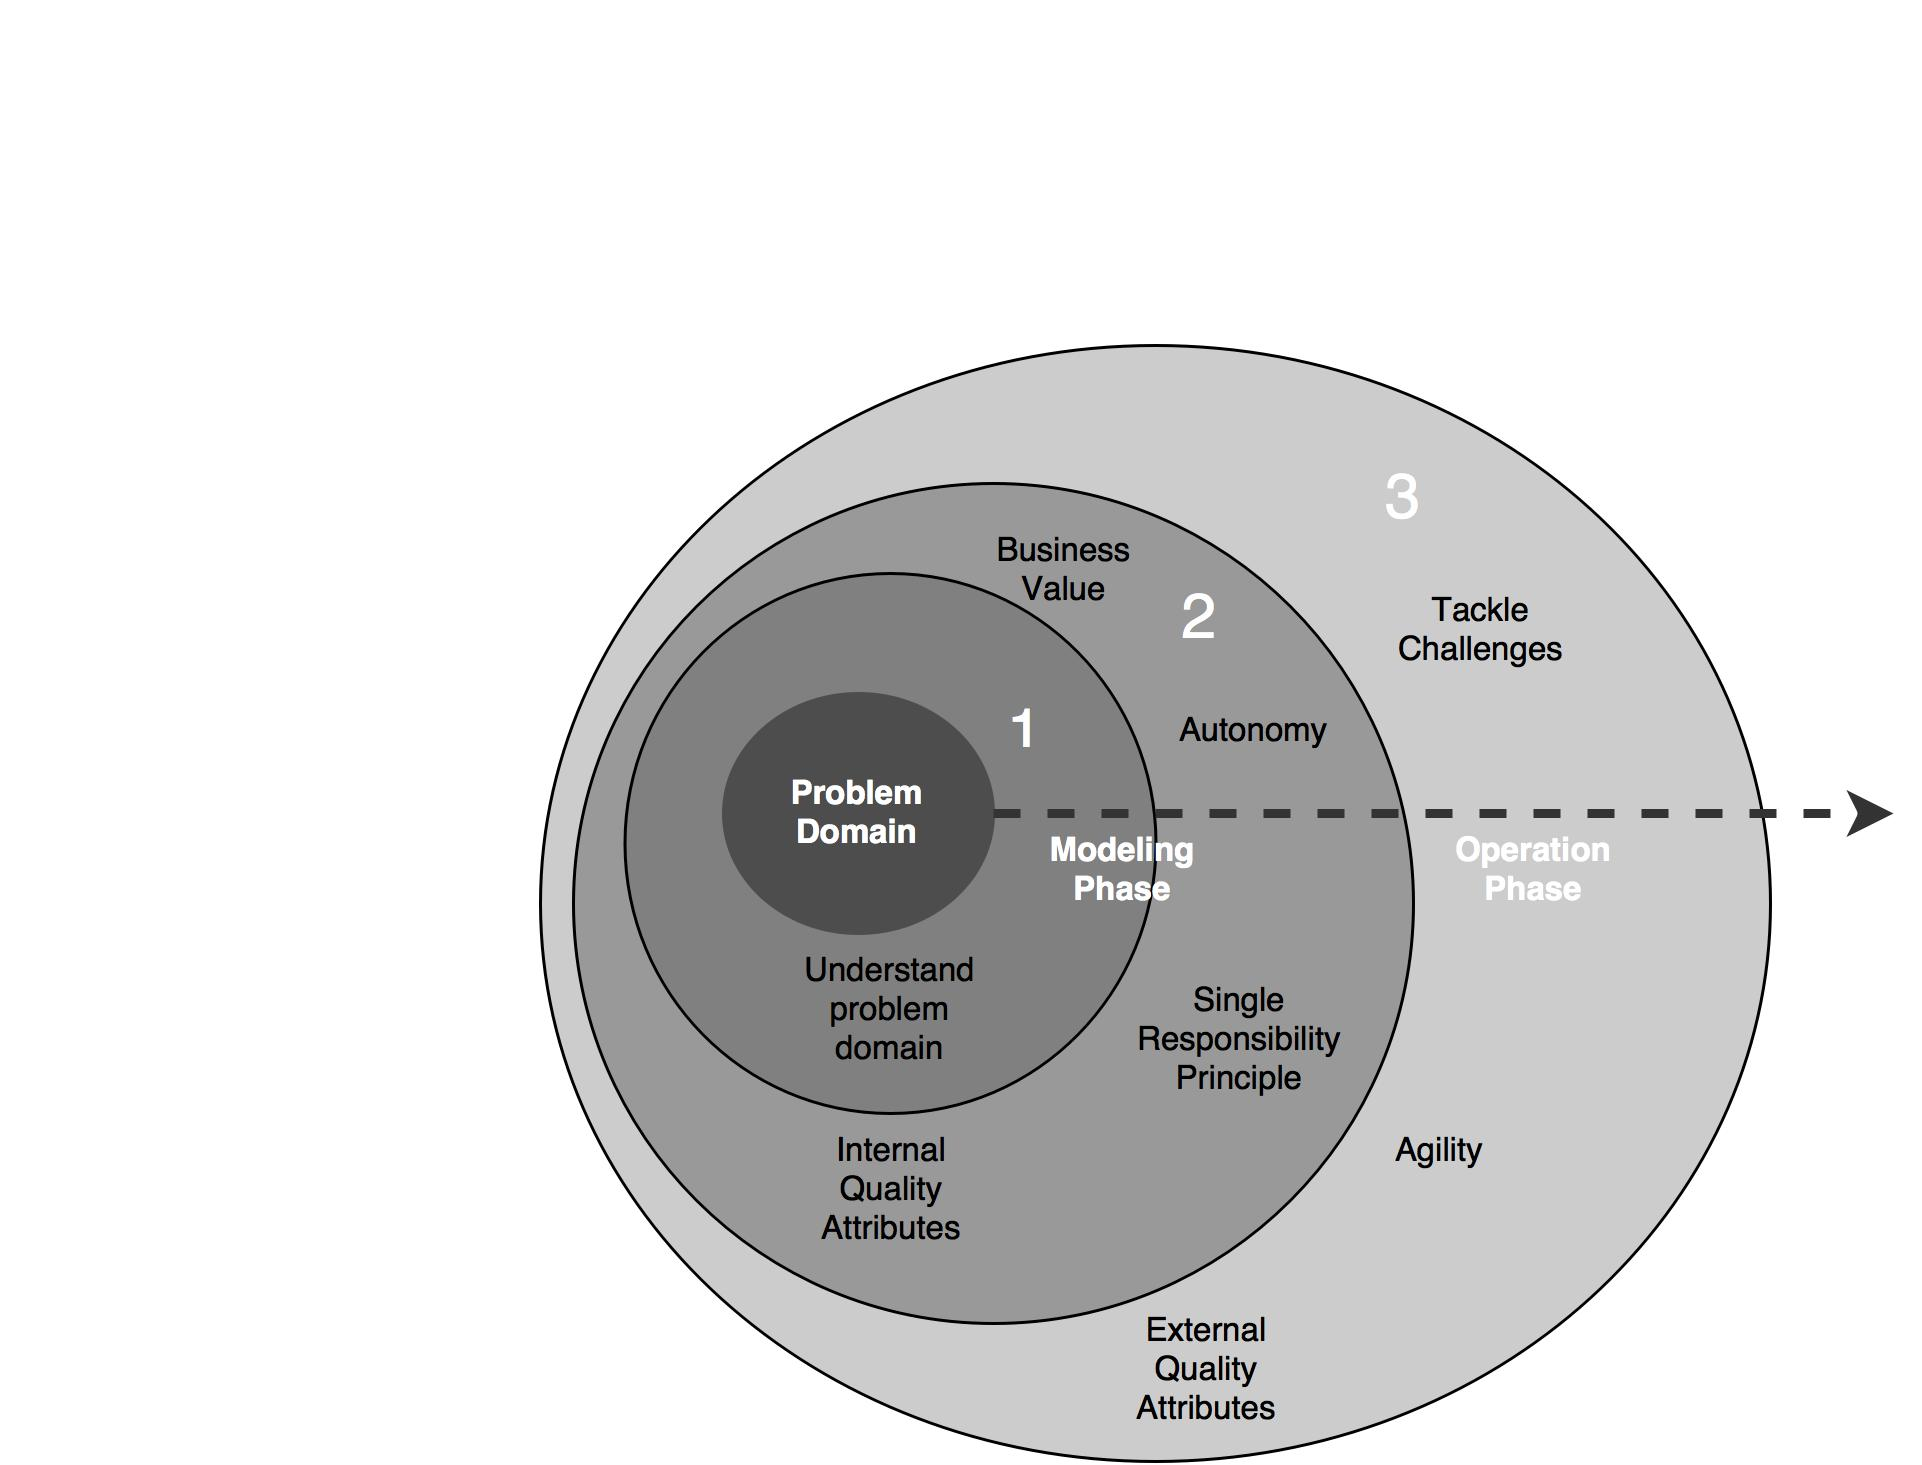
\includegraphics[width=0.7\textwidth]{figures/chapter_nine_process}
\caption{Process to implement microservices architecture}
\label{fig:guidelines/chapter_nine_process}
\end{center}
\end{figure}
\\
The microservices architecture follows a process which guides all the way from a) understanding the problem domain, b)  identifying modular components considering various attributes and c) implementing as well as operating the components to satisfy various external quality attributes. It is interesting to find how process, principles and guidelines are related. A process is based upon some basic principles and the principles helps to define guidelines based upon some specific requirements and environment. So, in order to understand the process of implementing microservices, it can be helpful to look into some basic principles.

\section{Principles And Guidelines}\label{section:guidelines/principles_and_guidelines}
Based upon the research findings as discussed in the previous chapters, various principles are listed to guide modeling microservices as well as operating them. It is highly recommended to follow these principles when considering microservices architectural approach.\cite{Newman:2015aa}
\begin{enumerate}
\item \textbf{Correct Granularity} \\
The dimension of granularity for microservice is given by a) the functionality it performs, b) data it handles and  c) the business value it provides \ref{section:granularity/dimensions}. These dimensions make it pretty obvious how to make the size of a service as low as possible. However, the notion of correct granularity is rather important and should be focused instead of trying to make the size as low as possible.\ref{section:granularity/principles} There are various factors which act together and tailor the size of the microservices.
\begin{enumerate}
\item One of the factors is \textbf{\acrshort{SRP}}, which influences the functionalities and data handled by microservices to make it as small as possible. \acrshort{SRP} encourages to focus on small set of cohesive tasks that change for the same reason. \cite{Stine:2014aa} \cite{Newman:2015aa} The influence of \acrshort{SRP} on the microservices architecture is also verified by the result of interview which is compiled in the Section \ref{section:hybris_architecture/interview/interview_compilation}.
\item Another important factor is \textbf{autonomy}. According to S. Newman, a microservice should be able to be deployed and updated independently \cite{Newman:2015aa}. Without any surprise, autonomy is an important quality attribute of the microservices and is evaluated as its degree of control upon the operations to act on its business entities \ref{section:quality_of_service/quality_metrics/autonomy}. As discussed in the Section \ref{section:granularity/principles}, a microservice should provide transaction integrity such that it is big enough to support the activities which fall under one transaction. So, autonomy tends to limit the scope of functionalities and data such that the microservice is a) self-contained, b) self-controlling and c) can be self-governed \cite{Ma:2007aa}.
\item The act of realizing the size of microservices as small as possible comes with a price. As the functionality of microservice is squeezed, the number of microservices needed for any application increases. The task of deploying, provisioning and governing these microservices can be challenging. So, as stated in the principles defined in the Section  \ref{principle:granularity/IT_infrastructure},  the decision regarding the size of service should be rational based upon the current \textbf{infrastructure and operational capability} to handle such large number of small microservices. It is further supported by the response of the interview compilation in the Section \ref{section:hybris_architecture/interview/interview_compilation}.
\item Finally, the size of microservices should also provide \textbf{business value} and should coincide with the business goal of the organization. It is also evident from the response of the interview compiled in the Section \ref{section:hybris_architecture/interview/interview_compilation}. Additionally, the business value being an important dimension of granularity of the microservices according to the Section \ref{section:granularity/dimensions}, should be examined at the design time while decomposing the problem domain.
\end{enumerate}

\item \textbf{Consider quality attributes as early as possible} \\
The internal quality attributes such as coupling, cohesion, autonomy, etc. should be controlled as early as possible during the modeling and development phases. Taking care of the internal quality attributes will eventually help to control the external quality attributes of the microservices such as reusability, reliability, resilience, etc. The Table \ref{tab:quality_of_service/quality_attributes/basic_quality_metrics} which identifies various basic metrics can be helpful to evaluate the quality of the microservices. For one thing, the metrics such as scope of opertions, number of operations, etc. used in the basic metrics table are completely in disposal to the developers and the teams of the microservices. Secondly, it helps to identify the relationship among them as shown in the Table \ref{tab:quality_of_service/quality_attributes/quality_attributes_relationship} and assists in managing trade offs when needed.

\item \textbf{Understand the problem domain}\\
As discussed in the Chapter \ref{chapter:service_candidate}, problem domain can be analyzed using either usecases refactoring approach or domain driven design approach. \\
Using usecases can break down the problem domain into various levels of abstractions, each abstraction representing lower scope of functionality. The graphical approach used in usecases modeling approach can be an effective approach for a) brainstorming, b) exploring the problem domain and c) finding new usecases.\\
Another popular approach is using domain driven design to explore the problem domain. The overall process looks natural and straight forward, which focus on dividing the complex problem domain into small manageable subdomains and further into modular autonomous components. Furthermore, the approach gives emphasis on using ubiquitous language to find autonomous modules and define their boundaries. The chapter \ref{chapter:service_candidate} provides important guidelines for finding ubiquitous language and bounded contexts.\\
The graphical approach provided by usecases are more familiar to architects as well as developers and thus can be faster. However, they tend to focus only on \acrshort{SRP} and scope of the functionalities. Following the process, may likely lose grip on very important quality attribute of the microservices called autonomy.\\
On the other hand, domain driven design with its approach of using ubiquitous language, focuses on autonomy. Additionally, by dividing the problem domain into smaller manageable components with limited scope, domain driven design also focuses on \acrshort{SRP}. Although the whole proces seems natural, getting the boundary right is a complex process. A clear understanding of the problem domain is necessary in order to get the bounded context right. So, it can be an iterative process, starting with bigger boundaries at first and down to smaller modular boundaries in several iterations.\\
The knowledge and practice of both usecases modeling and domain driven design can be helpful. Depending upon the complexity of the problem domain and experience with it, any of them or combination of them can be used to decompose the problem domain.

\item \textbf{Culture of Automation}\\
With such a large number of small services, the task of managing and operating them manually can become impossible. There are three specific areas where automation can serve greatly.
\begin{enumerate}
\item Automated Continuous Delivery can help building and deploying microservices frequently with consistency. Maintaining continuous integration and delivery pipeline can make sure that any new changes is consistent to old system and can be put into release in a matter of few button presses.
\item Automated Testing is another important area to consider when there are large number of microservices and large number of changes in the backlog. Without automated testing in the delivery pipeline, it can be hard deploy changes to release environment without breaking existing functionalities.
\item Infrastructure Automation and Provisioning should not be neglected either, especially when there can be different technology stacks in different microservices and different infrastructure environments. \acrshort{PaaS} such as CloudFoundry can be helpful for deployment and provisioning easily whereas various configuration management tools such as Puppet, chef etc can assist to manage different technology stacks.
\end{enumerate}
\item \textbf{Hide Internal Implementation}\\
Collaboration among the microservices is essential however high coupling by over exposing the inner-details should be avoided to save autonomy.
\begin{enumerate}
\item The first on the checklist is to model the \acrshort{API}s in right way. Rather than breaking the application into technological boundaries, the problem domain should be clearly understood to discover clear functional boundaries and should be modeled around business domains. The concept of bounded context can be a good approach to define clear \acrshort{API}s, which also reduces unnecessary coupling.
\item The \acrshort{API}s should be technology agnostic, which means that the technology used for collaborating between \acrshort{API}s should not guide the internal implementation of the \acrshort{API}s. Using \acrshort{REST} and some form of \acrshort{RPC} can be useful tackle them.
\item In microservices, database is also an integral part of internal implementation. Already mentioned in the Section \ref{section:challanges_of_microservices_architecture/integration/sharing_data}, sharing database tightly couples microservices as it exposes internal data structure details. In order to solve such coupling, each microservice should atleast have its own a) private tables,  or b) schema, or c) at most separate database server.
\item Additionally, in order to maintain loose coupling, the integration technology should be chosen carefully. As already discussed in the Section \ref{section:challanges_of_microservices_architecture/integration/inter_service_communication}, if business requirement allows, asynchronous communication styles such as a) publish/subscribe, b) notification, and c) request/async response should be chosen over synchronous request/response.
\end{enumerate}
\item \textbf{Decentralize} \\
Autonomy should not be limited to deployment and updates only. It should be applied in team organization as well. A team should be autonomous enough to own the microservices and control all the phases from a) developing the microservices, b) releasing them, and  c) maintaining in the production environment. In order to achieve that, the teams should be trained to become domain-experts in the business areas related to their microservices.
Additionaly, the architecture of microservices should follow decentralization as well. The business logic should be divided among microservices and should not be concentrated towards any specific a) god microservices and b) integration mechanism. The microservices should be smart enough to handle collaboration among themselves and the communication mechanism should be as dumb as possible such as \acrshort{REST} and messaging. Also, choreography should be highly applied whenever possible and orchestration should only be used if the business requirement dictates so.
\item \textbf{Deploy Independently}\\
Microservices should be able to be deployed independently. The Section \ref{section:challanges_of_microservices_architecture/integration/breaking_change} already discusses the challenges involved as well as their solutions.
\begin{enumerate}
\item In order to avoid breaking changes, a) the integration technology such as \acrshort{REST} should be used to decouple microservices and b) tollerant reader pattern should be used to implement consumers.
\item To find the breaking changes early during development, consumer-driven contracts should be implemented as automated tests in the delivery pipeline of the microservices. Additionally, semantic versioning can be used to clearly indicate the level of new changes.
\item When breaking changes cannot be avoided, maintaining co-existing endpoints with different versions or co-existing microservice versions can provide enough time and opportunity for consumers to get updated gracefully and without breaking \acrshort{API}s.
\item Finally, the release and the deployment can be decoupled using techniques such as bluegreen deployment \ref{section:appendices/blue_green_deployment} and canary release \ref{section:appendices/canary_release}, so that new changes can be tested in production with confidence and can be released later reducing the risk.
\end{enumerate}
\item \textbf{Consumer First}\\
The microservices are developed in order to serve its consumers, so consumers should be the priority when designing them.
\begin{enumerate}
\item \acrshort{API}s should be designed considering its consumers. It should be easy to a) understand, b) use and c) extend. The name as well as the link of \acrshort{API} should be self intuitive. Additionally, documentation to follow and use \acrshort{API} should be provided. In order help with these, there are various tools available such as swagger, RAML etc. The tools not only make it easy to design and document \acrshort{API}s but also provide capability to try them.\cite{Bloch:2016aa} \cite{Blanchette:2008aa}
\item Another important concept is to make it easy for consumers to find the microservices itself. There are various service discovery tools such as zookeeper, etcd, consul etc that can be used.
\end{enumerate}
\item \textbf{Isolate Failures}\\
The microservices are build on the top of distributed system and it is not false to say the distributed system cannot be perfectly reliable \cite{Factor:2014aa}. Although, with high number of the microservices and complex collaboration among them over unreliable network, the system should not be affected until all the microservices fail. The solutions are discussed in Section \ref{section:challanges_of_microservices_architecture/handling_failures}.
\begin{enumerate}
\item Timeout should be implemented realizing the fact that remote calls are different than local calls and they can be slow. A realistic value of timeout should be chosen based on the use cases scenario.
\item In order to avoid leaking failures and affecting the whole system as a result, bulkhead should be used to segregate the resources and an appropriate thereshold value should be maintained for each group of resources.
\item For reducing latency, circuit breaker should be implemented which detaches a failed node after certain attempts and reattemts automatically. In this way, it not only removes unnecessary roundtrip time or waiting time but also saves network resources.
\item Finally, fallback mechanism can be used in conjunction with timeouts and circuit breaker to provide alternative mechanism such as serving from cache, etc. In this way, it not only isolates the failures but also serves the request.
\end{enumerate}
\item \textbf{Highly Observable} \\
It can be difficult to observe the status of each microservice on each provisioned hosts considering the number of microservices. The Section \ref{section:challanges_of_microservices_architecture/monitoring} points out some ideas which can be used to make it easier.
\begin{enumerate}
\item Use semantic monitoring to check the current behaviour of the microservices such as availability, response time etc. An example of effective tools is uptime. Additionally, trigger certain tests to verify important logic of the microservices on regular basis. One way to achieve that is to trigger smoke tests automatically.
\item In order to get the overall picture of the whole application at one place, use logs aggregation and visualization tools such as logstash and kibana.
\item Finally, use correlation ids to get a semantic picture of the related requests which gets branched out along many downstream microservices.
\end{enumerate}
\end{enumerate}